\documentclass[11pt]{article}
\usepackage{../EllioStyle}
\usepackage{fancyvrb}
\usepackage{pdfpages}
\usepackage{xcolor}


\usepackage{fancyvrb}

% redefine \VerbatimInput
\RecustomVerbatimCommand{\VerbatimInput}{VerbatimInput}%
{fontsize=\footnotesize,
 %
 frame=lines,  % top and bottom rule only
 framesep=2em, % separation between frame and text
 rulecolor=\color{gray},
 %
 label=\fbox{\color{black}design pattern finder output.txt},
 labelposition=topline,
 %
 commandchars=\|\(\), % escape character and argument delimiters for
                      % commands within the verbatim
 commentchar=*        % comment character
}


\title{Homework 5}
\author{Elliott Pryor}
\date{5 Nov 2020}


\begin{document}
\maketitle


\problem{1}
\subsection*{A}

\begin{enumerate}[1.]
	\item What system did you download? I downloaded BoardGame Bay 
	\url{https://sourceforge.net/projects/gamebay/files/gamebay_chess_0.7/}
	which is a Chess game. 
	
	\item What does it do? It is a chess simulator. So players can play chess using it.
	
	\item How many Lines of Code does it have? How did you calculate this? This has 5187 lines of code. I wrote a python script that walks through the directories and opens all the .java files and counts the lines. 

\end{enumerate}

\subsection*{B}

\begin{enumerate}[1.]
	\item 
	
	\VerbatimInput{data.txt}
	
	\item Since we did not use the `Search in File Content' option it looks at the file name. So it is only guessing the design pattern by the filename. So it relies on standard conventions such as naming factory classes with the name Factory. If we had checked this option it would presumably scan through each file and look for similar conventions.
	
	\item I think that this method works. 
	It is not very intelligent at actually detecting the design patterns.
	 This algorithm relies entirely on standard naming conventions. 
	 So it would not detect it if you were to rename variables or use different conventions it would not work.
	  But, this is the only practical way that I can think of to implement this. It is not feasible or practical to write an algorithm to analyze code structure intelligently in order to detect all of these cases. 
	  Perhaps it is possible with some complicated pattern matching and machine learning. But this is too computationally expensive. 
	I would also implement something that was based on naming conventions as it can quickly give an overall picture of what is happening under the hood.
\end{enumerate}




\problem{2}

\begin{figure}[H]
    \centering
    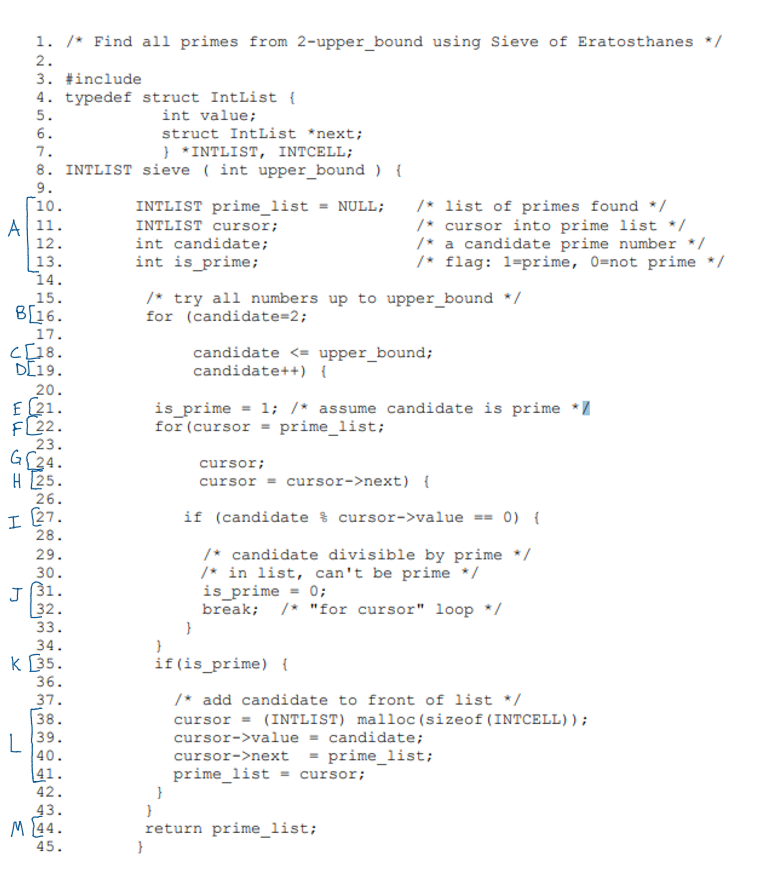
\includegraphics[scale = 0.5]{./q2.png}
    \caption{Labeled Nodes in Code}
    \label{fig:nodes}
\end{figure}

\begin{figure}[H]
    \centering
    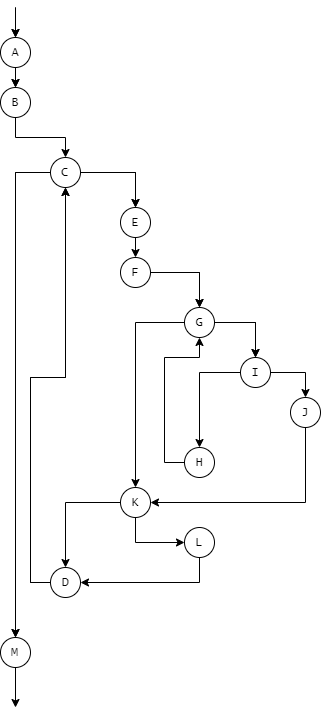
\includegraphics[scale = 0.5]{./CFG_Prob2.png}
    \caption{Control Flow Graph}
    \label{fig:cfg}
\end{figure}

\begin{enumerate}[a)]
	\item upper\_bound = 50, sieve(50). This tests all the nodes (and edges). The set $2... 50$ contains primes and non-primes so at least one candidate will trigger each node
	
	\item upper\_bound = 50, sieve(50). As mentioned in a) this tests all edges. Any test set that contains one prime and one non prime will cover all edges. Also in this case, node coverage is equivalent to edge coverage since it is not possible to cover all the nodes without using all the edges. The only edge that could be skipped is $G \rightarrow K$ which is not possible to have a set that does this since you can't have a list of numbers $2..x$ that is only non-primes so transition $J \rightarrow K$ must not be used for at least one candidate.
	
	\item No this is not possible in general. There could be infinite inputs or non-reachable segments of code, so these non-reachable segments could never be covered by any test case. 
	

\end{enumerate}


\problem{3}

\begin{enumerate}[a)]
\item 
\begin{figure}[H]
    \centering
    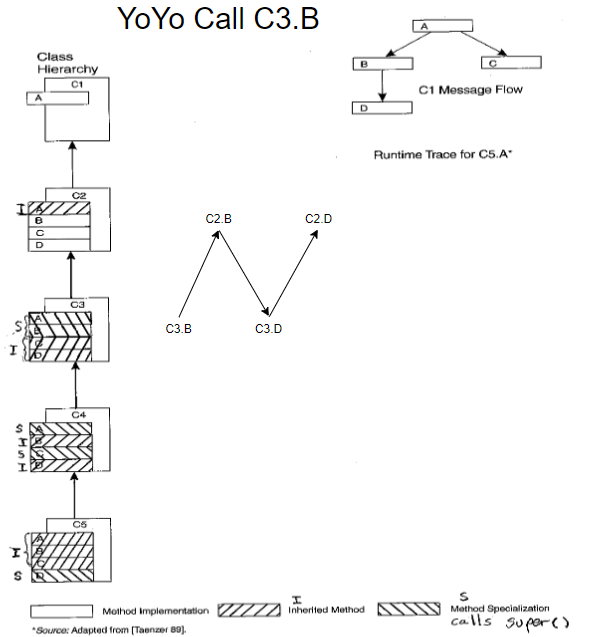
\includegraphics[scale = 0.7]{./q3a2.png}
    \caption{Yo Yo call from C3.B}
    \label{fig:yoyo1}
\end{figure}

\begin{figure}[H]
    \centering
    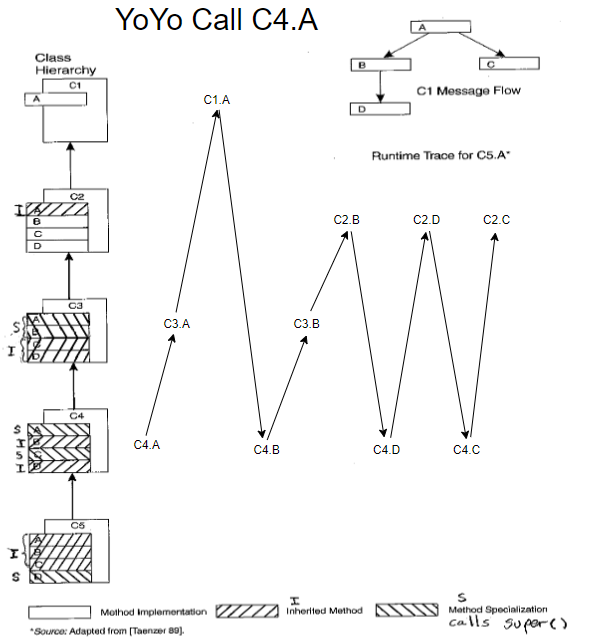
\includegraphics[scale = 0.7]{./q3a1.png}
    \caption{Yo Yo call from C4.A}
    \label{fig:yoyo2}
\end{figure}



\item It errors as class C1 does not have method D

\end{enumerate}



\problem{4}

\begin{enumerate}[a)]

	\item input = 1 $\implies$ return 0 instead of 1
	
	\item input = 0 $\implies$ return 0 instead of 1
	
	\item input = 5 $\implies$ return 16 instead of 8

\end{enumerate}

\end{document}